\chapter{Employing GPUs in scientific algorithms}
\label{chap:gpu}


This chapter summarizes the process of porting several specific scientific algorithms to GPUs and uses these to exemplify the challenges of optimizing for GPU architectures.

\section{Hierarchical clustering with the Mahalanobis linkage}
\label{sec:maha}

Hierarchical clustering is an unsupervised machine learning method that aims to group the data points into clusters according to some \emph{linkage criterion}.
In the domain of bioinformatics, hierarchical clustering with the \emph{Mahalanobis linkage} is used, which is a more sophisticated method suitable for analyzing multidimensional single-cell cytometry datasets.

Mahalanobis linkage, proposed by Fišer et al.~\cite{fivser2012detection}, allows for a very natural formation of clusters in biological data. However, the benefits come at a cost of high time and space complexity. The authors claim the upper usable bound of dataset size to be $10^4$ using the original \texttt{C} application. They state that the quadratic space complexity makes for the most significant limiting factor, leaving it unfeasible to analyze bigger datasets on current desktop computers.

\subsubsection{Algorithm complexity}

Mahalanobis linkage uses \emph{Mahalanobis distance}~\cite{mahalanobis1936generalized} to measure the similarity between clusters:
\begin{defn}[Mahalanobis distance]
    Suppose a probability distribution $C$ on $\R^d$ with mean $\bar{C} \in \R^d$ and a covariance matrix $\cov(C)$. If the matrix $\cov(C)$ is regular, we define the \emph{Mahalanobis distance} between $u \in \R^d$ and $C$ as
    \begin{equation}
    d_\text{Maha}(u,C) = \sqrt{(u-\bar{C})^T\cov(C)^{-1}(u-\bar{C})}.
    \end{equation}\label{eq01:maha}
\end{defn}

To illustrate the measure of the Mahalanobis distance, let us suppose we have two elliptic clusters. In the means of proximity, the measure favors such clusters that their ellipses are alongside rather than in a prolongation of one another~\cite{dagnelie1991using}.
Only when the objects of a cluster form a spherical shape, this dissimilarity measure is proportional to the Euclidean distance with a corresponding linkage (as depicted in Figure~\ref{fig:ellipses}).

\begin{figure}[h]
    \centering
    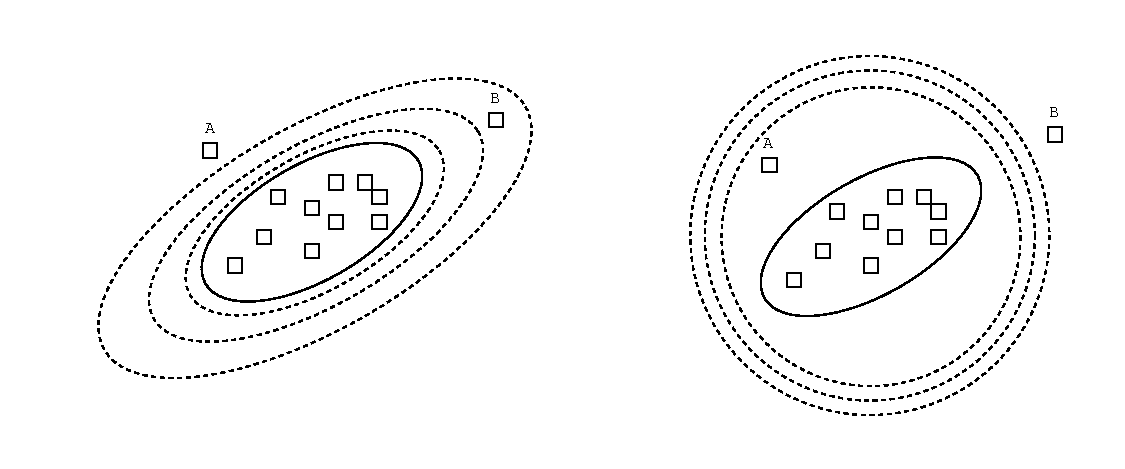
\includegraphics[width=0.8\textwidth]{img/maha.pdf}
    \caption{A comparison of the Mahalanobis (left) and Euclidean (right) distance in the context of elliptic clusters. The contour lines represent the space of the equal distance from the cluster centroid.}
    \label{fig:ellipses}
\end{figure}

The standard Hierarchical Clustering (HC), which utilizes a dissimilarity matrix, has a time complexity of $\mathcal{O}(n^3)$ and space complexity of $\mathcal{O}(n^2)$. There are other variants of HC which use a different method for the closest cluster pair retrieval and the amount of distances to recompute after each iteration. Other variants include HC with the nearest neighbor array, which trades the linear memory complexity for a worse time complexity on average, or the HC with priority queues, which reduces the time complexity to $\mathcal{O}(n^2 \log n)$ for the sake of bigger memory requirements~\cite{day1984efficient}.

\subsubsection{Implementation}

From the perspective of GPU programming, Mahalanobis HC is a challenging problem. Algorithms with high memory requirements are generally unfavorable for GPUs due to limited availability of global memory (refers to \nameref{sec:memory_hier} in \cref{sec:gpu_optim}). There has been a lot of work on overcoming this limitation, both from NVIDIA and the scientific community~\cite{zheng2016towards,kim2020batch,landaverde2014investigation}: CUDA has introduced \emph{unified memory}~\cite{site:cuda}, which allowed GPUs to work on data that exceeds GPU memory capacity by seamlessly copying data from CPU to GPU on page fault. This optimization can help only to a certain extent, as it can only scale to the size of CPU RAM and the data are usually sent through high-latency small-throughput interconnect (refers to \nameref{sec:transfers} in \cref{sec:gpu_optim}). Therefore, in our work, we experimented with other well-known HC variants that trade higher time complexity for a linear memory complexity --- \emph{HC with the nearest neighbor array}~\cite{day1984efficient}.

The other obstacle present in Mahalanobis HC is the greatly imbalanced workload. In the first iterations, the runtime is dominated by the complex Mahalanobis linkage computation over many pairs of $n$ clusters. But as the number of clusters decreases, the hot spot moves to the computation of the covariance matrix of a merged cluster. A naive implementation would thus leave the GPU significantly under-utilized, either because of small amount of parallelism in covariance matrix computation or in the similarity computation. To alleviate this issue, we designed a workload that uses CUDA \emph{streams} (refers to \nameref{sec:transfers} in \cref{sec:gpu_optim}), which enabled running these tasks in parallel. Consequently, this allowed us to keep the utilization of GPU cores high during the whole runtime of the algorithm.

\subsubsection{Results}

The optimized Mahalanobis HC achieves a speedup of over $1400\times$ compared to the original serial CPU implementation. We benchmarked the application on the real-world single-cytometry datasets. The biggest dataset which we benchmarked, the Samusik-All~\cite{flowrepo} ($841$ thousand $39$D points), was able to finish in the order of minutes compared to the order of days. Furthermore, we have packaged and distributed the application as a R package \texttt{gmhc} to fit workflows carried out by the bioinformatics community. To the best of our knowledge, the package enabled the scientists to analyze big datasets as a whole, increasing the accuracy of the analyzed data and decreasing the turnaround time of the analysis.




\section{Neighborhood-based dim. reduction}
\label{sec:embedsom}


Complementary to hierarchical clustering, a different approach to displaying cytometry datasets is \emph{dimensionality reduction} (also called \emph{embedding}), in which multidimensional cells are projected into a 2-dimensional plane, a picture, which shows cells arranged in groups with common properties.

The currently used dimensionality reduction tools are typically based on the principle of optimizing a low-dimensional embedding while preserving high-dimensional properties of interest. However, the most popular tools following this methodology, such as t-SNE~\cite{maaten2008visualizing}, UMAP~\cite{becht2019dimensionality} or TriMAP~\cite{amid2019trimap}, can suffer poor performance on large data due to the need to examine a nontrivial subset of $\binom{n}{2}$ relations (such as the pairwise distances) between $n$ data points~\cite{kratochvil2019generalized}. \emph{EmbedSOM} algorithm, introduced by Kratochvíl et al.~\cite{kratochvil2019generalized}, is designed to overcome this limitation. The costly parts of the previous methods can be omitted by creating a smaller model of the data obtained by \emph{self-organizing maps}. EmbedSOM uses the information of such an approximated manifold to compute the final embedding, retaining a competitive quality of the visualization.

Let us overview the EmbedSOM algorithm. It assumes a set of $n$ high-dimensional points $X \in \R^{n \times d}$ and the smaller data model: a set of $g << n$ high-dimensional landmarks $L \in \R^{g \times d}$, and a set of $g$ low-dimensional landmarks $l \in \R^{g \times 2}$. For each input point, $k < g$ nearest landmarks from $L$ are found and assigned scores according to their distance. Finally, we compute the embedding such that the difference between distances from $l$ landmarks and the embedded point and $L$ landmarks and the original point is minimized. The minimization problem is reducible to a linear system of equations with two variables.

\subsubsection{Interactive opportunities of GPU implementation}

The main challenge of EmbedSOM is low \emph{arithmetic intensity} (refers to \nameref{sec:arithmetic_int} in \cref{sec:gpu_optim}). For GPUs, there are many ways to fight the arithmetic intensity of an algorithm, such as kernel fusion~\cite{wahib2014scalable}, leveraging the memory hierarchy~\cite{lee2012cuda} or by reordering data accesses~\cite{ghysels2012improving} and optimizing data transactions~\cite{lu2020optimizing}. Generally, these approaches can be distilled into two groups: \emph{Data sharing} and \emph{latency hiding} (refers to \nameref{sec:memory_hier} and \nameref{sec:occupancy} in \cref{sec:gpu_optim}).

We experimented with both approaches in our EmbedSOM implementation. Although L2 caches can partially handle data sharing, GPUs typically hardly benefit from them due to their low cache-to-core ratio~\cite{site:cuda}. Therefore, as one variant of $k$-NN part, we used \emph{shared memory}, a programmable cache, to store the data and landmarks. These were then used to compute all the possible pairwise distances before loading the next batch to maximize the arithmetic intensity. The second variant of the $k$-NN part used a modified \emph{bitonic sort} to find the top-$k$ landmarks. This approach has the hidden benefit of low per-thread resource requirements, resulting in higher maximum GPU occupancy and, consequently, better latency hiding (refers to \nameref{sec:occupancy} in \cref{sec:gpu_optim}).

The embedding part of EmbedSOM does not offer such caching opportunities, as each point has a different set of nearest landmarks. The only reuse can happen on the landmarks themselves. And since their count can be limited in some parameter configurations, we experimented with techniques that increase the memory bandwidth, such as \emph{vector load instructions}.

\subsubsection{Results}

Using the aforementioned optimizations, we increased the performance by $200-1000\times$ over the serial CPU version and $3-10\times$ over a na\"{i}ve GPU implementation. Furthermore, the achieved speedup enabled the interactive data visualization and was integrated into the graphical application \emph{BlosSOM}~\cite{molnarova2023throughput}. Thanks to the improved performance, the application can project datasets of up to a million points with a maintained frame rate above $30$ frames per second on consumer hardware. This contribution pushes the boundary of EmbedSOM into a semi-supervised dimensionality reduction domain, allowing users to effectively and intuitively visualize data with real-time feedback.


\section{Cross-correlation optimized for small inputs}
\label{sec:cross-correlation}

Leaving the realm of cytometry data analysis, we will focus on a highly data-bound problem: cross-correlation. This algorithm is a cornerstone of many scientific fields, such as image processing, seismology, material physics, and, with the advent of convolutional neural networks, machine learning.

The problem of cross-correlation performance was initially introduced to us by the physicists from the Department of Physics of Material at Charles University in Prague. They used the algorithm to analyze the diffraction pattern of metallic alloys from electron backscatter diffraction (EBSD) cameras to obtain the material \emph{deformation}. That can be used to study the material characteristics, such as elastic strain or lattice rotation.

The reference Python script provides the physicists with the computational throughput of tens of patterns per second. However, modern EBSD cameras produce data at a magnitude higher rate~\cite{bali2021zpracovani}. Nevertheless, thanks to the parallel nature of the problem, this is a perfect candidate for GPU acceleration.

\subsubsection{Implementation challenges}

The cross-correlation of functions $f, g: \mathbb{C}\rightarrow \R$ is defined as
\begin{equation}
    (f \star g)(\tau) = \sum_{i=-\infty}^{\infty} f(i) g(i+\tau).
\end{equation}
Figure~\ref{fig:cross-correlation} depicts the visual representation of the equation applied on a discrete case of two $2\times 2$ matrices. The matrices are shifted to produce all the possible overlaps (Figure~\ref{fig:cross-correlation}, right). For a single shift, only overlapping elements contribute to the computation: overlapped pairs are multiplied and summed together into a single output matrix element (Figure~\ref{fig:cross-correlation}, left).

\begin{figure}
    \centering
    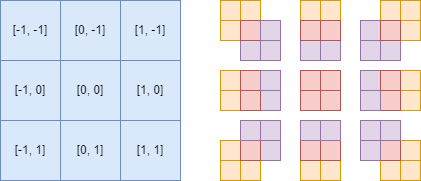
\includegraphics[width=0.6\textwidth]{img/cc.png}
    \caption{Visual representation of the cross-correlation. Yellow and purple matrices correspond to the input matrices, and the blue matrix depicts the cross-correlation output. The coordinates on the blue matrix correspond to the shift of the yellow matrix, which is depicted on the right. Only the overlapping parts (in pink) contribute to the computation for each output matrix element.}
    \label{fig:cross-correlation}
\end{figure}

For general $w \times h$ matrices, the cross-correlation has a time complexity of $\mathcal{O}(w^2 \cdot h^2)$. Alternatively, the input can be modified and passed to the Fast Fourier Transform (FFT) with a more pleasing time complexity of $\mathcal{O}(w\cdot h \cdot \log(w\cdot h))$. However, the hidden multiplicative factor, which materializes as an overhead in the implementations of FFT, favors the original, definition-based approach for small problem sizes.

\subsubsection{Optimization techniques}

Assesing a na\"{i}ve algorithm, its arithmetic intensity equals to $\frac{n}{2n * 4} = \frac{1}{8}$ for single-precision floats. With this in mind, we experimented with extreme data reuse techniques. There are many opportunities where the same data is read multiple times: When computing neighboring overlaps, most data from left and right matrices are read multiple times. As another possibility, in the $1:N$ or $N:M$ scenario, when cross-correlating one or multiple left matrices with many right matrices, a piece of data can be read once to compute multiple overlaps.

In order to reuse data, threads need to have them stored in the registers. The number of registers is limited, and the compiler can spill the data into slower memory if the limit is reached. Also, if the amount of resources per thread is high, the occupancy of the GPU can drop, and the achievable performance can decrease. The other big issue is the parallelism. Naturally, if one worker performs multiple operations for the sake of sharing, the parallelism decreases. Therefore, the most effective implementation maintains the optimal balance between data sharing and parallelism.

\subsubsection{Results}

The final implementation of the cross-correlation algorithm achieved a speedup of $5-10\times$ over a na\"{i}ve GPU code. The benchmark also uncovered the boundaries, above which a more expensive time complexity of the definition-based algorithm overcomes the overhead of the FFT approach. In summary, achieved speedup can enable physicists to analyze the data at a similar rate as EBSD cameras produce.


\section{Stochastic simulation of Boolean networks}
\label{sec:maboss}


In Systems biology, the analysis of large and complex biological systems is a challenging task. \emph{Boolean models}~\cite{wang2012boolean} have gained popularity due to their simplicity, scalability, and ability to describe complex signaling networks. A Boolean model consists of $n$ nodes with binary values --- active or inactive. A node represents an event in the system, such as a gene being expressed or a protein being activated. The complete state of the system is, therefore, defined by a Boolean word composed of $n$ bits. The states can transition within each other based on $n$ Boolean formulae, one for each node. Given an initial state, the task of the model is to predict the probability distribution of system outcomes after a specified amount of time.

Numerical methods, such as ExaStoLog~\cite{koltai2020exact}, have been developed and used to solve Boolean models; however, they are limited to relatively small models (tens of nodes) due to the exponential memory requirements. For larger models, it has proved to be much more efficient to approximate the results by simulation. A C++ software, MaBoSS~\cite{stoll2017maboss}, simulates these systems by applying the kinetic Monte-Carlo algorithm~\cite{stoll2012continuous} on the Boolean network. In summary, the MaBoSS tool simulates millions of random walks (also called the \emph{trajectories}) on the state space of the Boolean network (a directed weighted graph). The trajectories are then aggregated in a histogram-like fashion to compute various statistics, such as the probability distribution of the states over time, as is shown in Figure~\ref{fig:maboss}.

Due to the stochastic nature, this approach can overcome the limitations of numerical methods and has enabled the analysis of bigger models, running instances with a few hundred nodes in a reasonable amount of time. On the other hand, allowing even bigger inputs would require billions of simulated trajectories in order to obtain a reliable result, which puts significant pressure on the tool and its ability to scale well. A parallel CPU MaBoSS simulation of a relatively small Sizek model~\cite{sizek2019boolean} ($n=93$) with $10^6$ trajectories takes the order of minutes on a high-end computer. Simulating models with thousands of nodes and billions of trajectories would require an order of days in runtime, hindering further analysis of the models.

\begin{figure}
    \centering
    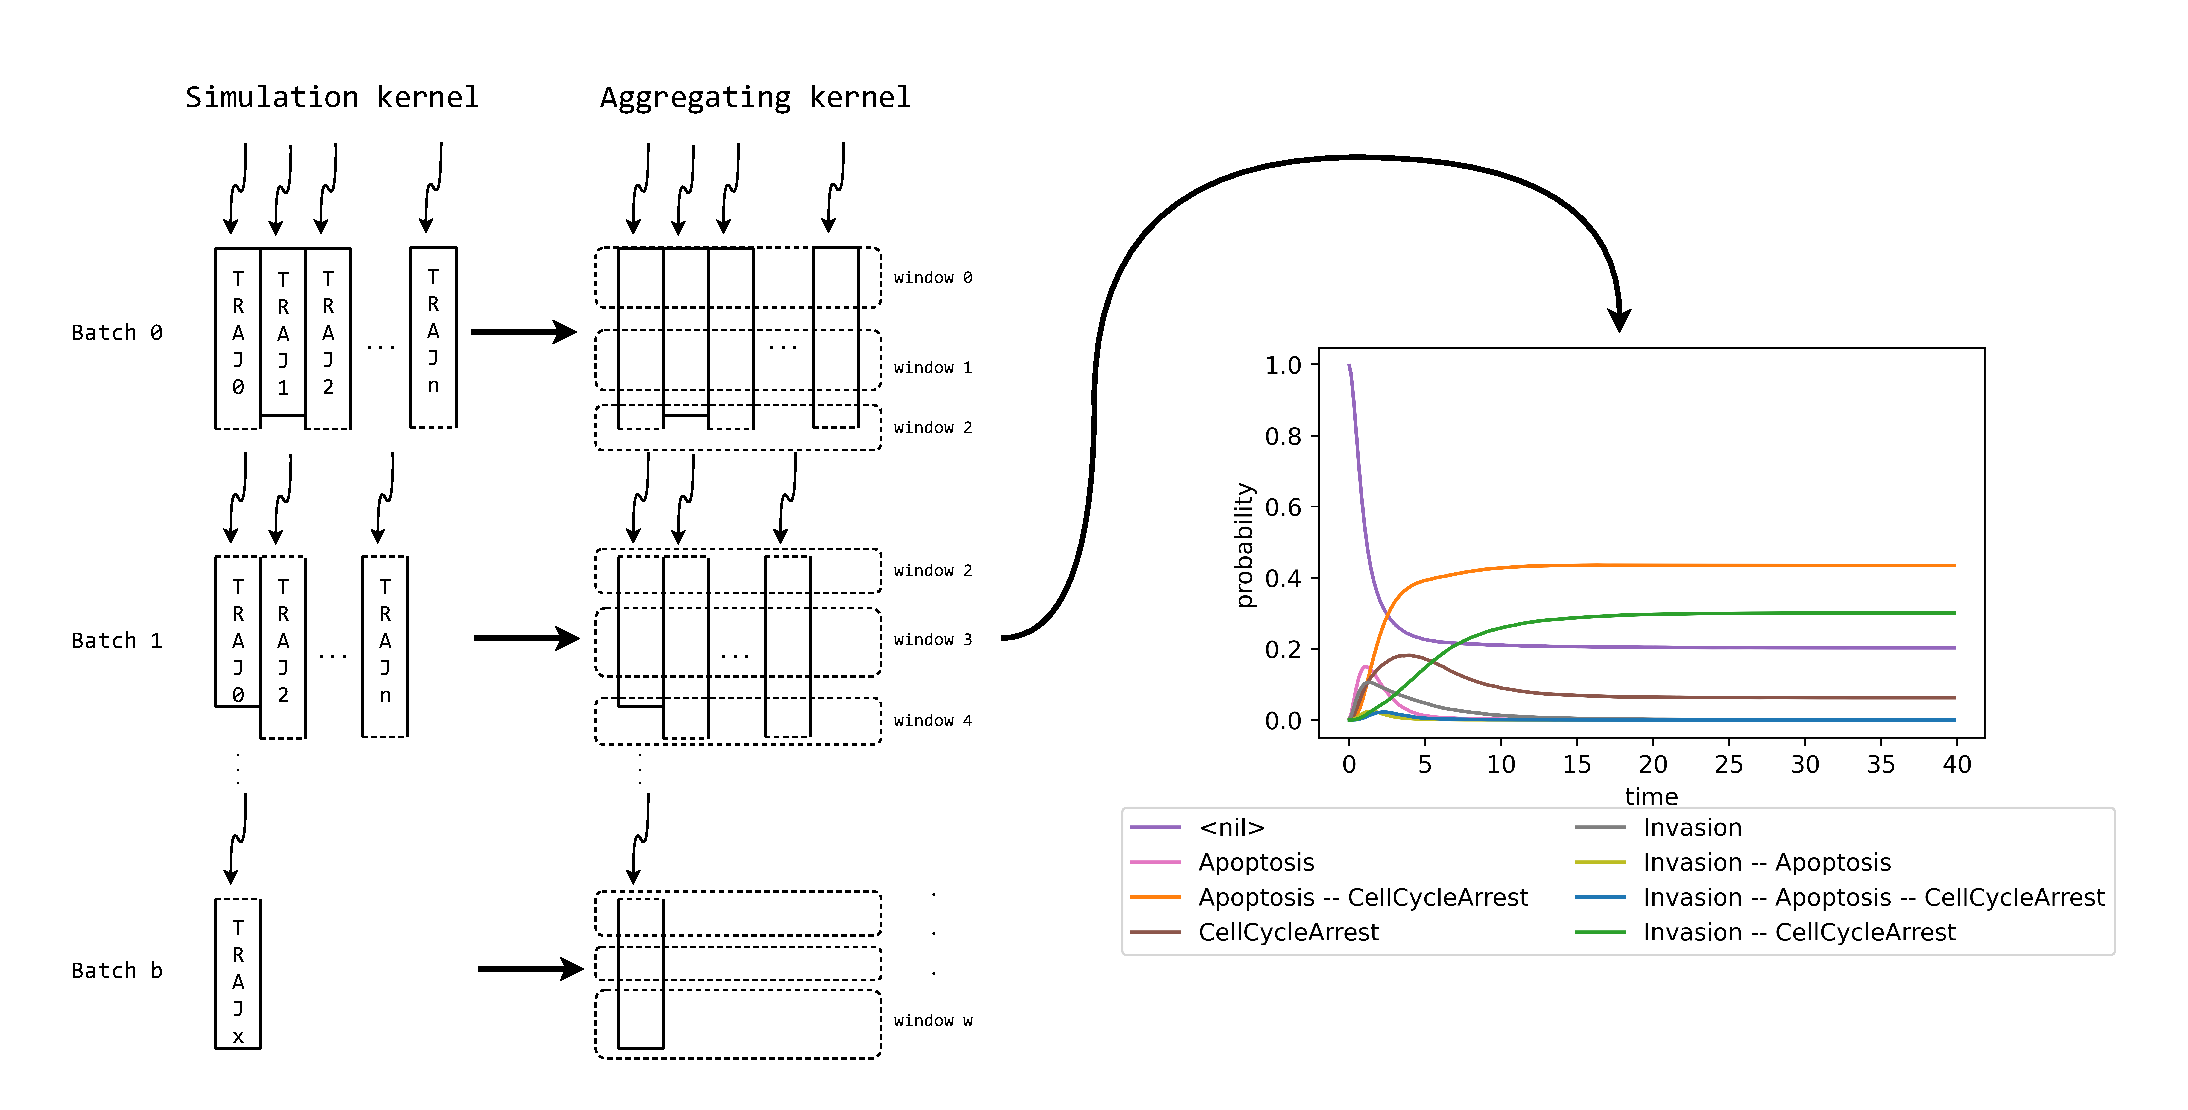
\includegraphics[width=\textwidth]{img/mabossg-kernels.pdf}
    \caption{The MaBoSS projection of simulated trajectories averaged over a specific time window.}
    \label{fig:maboss}
\end{figure}

\subsubsection{GPU acceleration challenges}

Although the parallelization of MaBoSS may seem straightforward, it includes challenges that can significantly affect the overall performance. The main issue is the traversal of the binary expression tree to evaluate the Boolean formulae requred to sample transition probabilities. Generally, traversing irregular data structures causes conditional branching and creates an irregular data access pattern (refers to \nameref{sec:divergence} and \nameref{sec:coalescing} in Section~\ref{sec:gpu_optim}). A combination of these issues may leave GPU heavily underutilized, gaining very little to no performance improvement over a well-parallelized CPU code.


In our work, we used the \emph{CUDA NVRTC}~\cite{nvrtc-online} runtime compilation library to compile the formulas on the fly. It has the benefit of encoding the formulas into a native binary code, removing the necessity to fetch the data from the memory each time the formula is evaluated. Apart from that, the compiler can run a set of optimizations on the code, further improving the performance. Consequently, the runtime compilation comes at the cost of an additional runtime. Thankfully, our benchmarking showed that the compilation time amortizes well for simulations with reasonably big inputs.

\subsubsection{Results}

The final implementation of the MaBoSS simulation achieved a speedup of $100-300\times$ on real-world datasets over the parallel CPU version. Moreover, we created a synthetic test suite to stress the scalability of the implementation, which showed that the GPU implementation can simulate models with thousands of nodes and billions of trajectories in minutes. These results suggest that the consumer laptop equipped with a GPU can simulate models that were previously restricted to high-end computers. Furthermore, the double and triple mutant analysis no longer belongs just to the domain of supercomputers but could become feasible on data center-grade GPUs. Overall, we believe that the GPU acceleration of the MaBoSS simulation can significantly improve the analysis of Boolean networks and enable researchers to explore complex models while conveniently using their personal computers.

\section{Summary}

This chapter presented the work of implementing four scientific algorithms in the HPC domain. Overall, the results have shown that employing GPUs to solve scientific problems can help researchers push the boundaries of the size, scale, and complexity of analyzed data while leveraging the computational power of their GPU-equipped personal computers or laptops.

Further summarizing the optimization used, it comes as no surprise that the most important aspect to consider when designing an optimized implementation is memory. Memory complexity, memory access patterns, memory hierarchies, and data caching repeatedly occurred in our implementation designs and have contributed the most to performance improvements.

Therefore, we dedicate the second chapter of this thesis to the methods for streamlining memory-related optimizations, which we collected during our optimization efforts and found them to be effective in aiding HPC programmers in writing optimized CPU or GPU code from scratch.

